\documentclass{article}
\usepackage[T1]{fontenc}
\usepackage{lmodern}
\usepackage{graphicx}
\usepackage{amsmath,amssymb}
\usepackage[a4paper,margin=2cm]{geometry}
\usepackage[absolute,overlay]{textpos}
\setlength{\TPHorizModule}{1mm}
\setlength{\TPVertModule}{1mm}
\usepackage[indonesian]{babel}
\usepackage{hyperref}
\setlength{\emergencystretch}{2em}
% unit: Halaman 7

\begin{document}

% === Halaman 7 (python/native) ===

7

• Top 10 huruf yang sering muncul dalam teks 

Bahasa Inggris: E, T, A, O, I, N, S, H, R, D, L, U 

• Top 10 huruf bigram yang sering muncul dalam 

teks B. Inggris: TH, HE, IN, EN, NT, RE, ER, AN, TI, 

dan ES 

• Top 10 huruf trigram yang sering muncul dalam 

teks B. Inggris: THE, AND, THA, ENT, ING, ION, 

TIO, FOR, NDE, dan HAS 

• Kriptanalis menggunakan tabel frekuensi 

kemunculan huruf dalam B. Inggris sebagai 

kakas bantu melakukan dekripsi.

• Misalnya, jika huruf “R” paling sering muncul di 

dalam cipherteks, maka kemungkinan besar itu 

adalah huruf “E” di dalam plainteksnya.

% deskripsi: gambar native xref 53
\noindent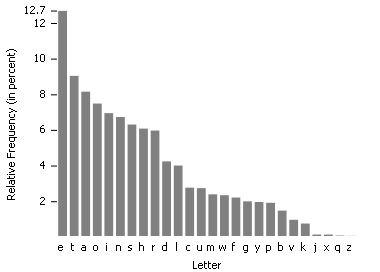
\includegraphics[width=0.85\textwidth]{../../images/python/page_007_img_01.png}

\end{document}
